To illustrate the structure of our implementation, in
\Cref{sub:jolie_extensions} we discuss how media and protocols are separated
from the Jolie interpreter and available as independent libraries. Then we
describe the highlights of the implementation of UDP and CoAP in
\Cref{sec:impl_coap_udp} and of MQTT in \Cref{sub:impl_mqtt}.

\subsection{Programming a Jolie Extension}
\label{sub:jolie_extensions}

In Jolie the implementations of the supported application and transport
protocols are independent. This enables the composition of any transport
protocol with any application protocol. Concretely, the Jolie language is
written in Java and provides proper abstract classes that represent
application and transport protocols. Each protocol is obtained as an
implementation of the corresponding abstract classes. Each implementation is a
separated library which is loaded only if the protocol is used. This expedites
the integration of new protocols in the language.

To better illustrate this structure, we report in \cref{fig:comm_modules} a
conceptual representation of the call flow that originates from the execution
logic of the language and interacts with the external libraries present in a
given installation. The flow starts from the Execution Engine, which
interprets Jolie commands, and which is the originator of the communication
flows. This is represented by arrow \circled{0} from the Execution Engine.
From there, the call reaches the Communication Core, which implements the
generic logic of channel creation, in turn relying on the pairing of a medium
and a protocol. In the interpreter, this division is generalized with abstract
factories for media and protocols. At runtime, the Communication Core proceeds
(arrows \circled{1}) to load the medium factory requested in the call from the
Execution Engine---in the figure we assume this is Socket---and, from that, it
obtains an implementation of the actual logic of a TCP/IP channel, which
includes a Communication Channel for managing outbound communications and a
Listener for managing inbound communications. Finally, the Communication Core
associates (arrows
\circled{2}) a protocol to the obtained medium. The flow is similar to that of
media: the Communication Core loads the protocol factory requested in the call
from the Execution Engine---in the figure we assume this is HTTP---and, from
that, it obtains an object that implements the logic of the HTTP
protocol.

\begin{figure}[t]
  \centering
  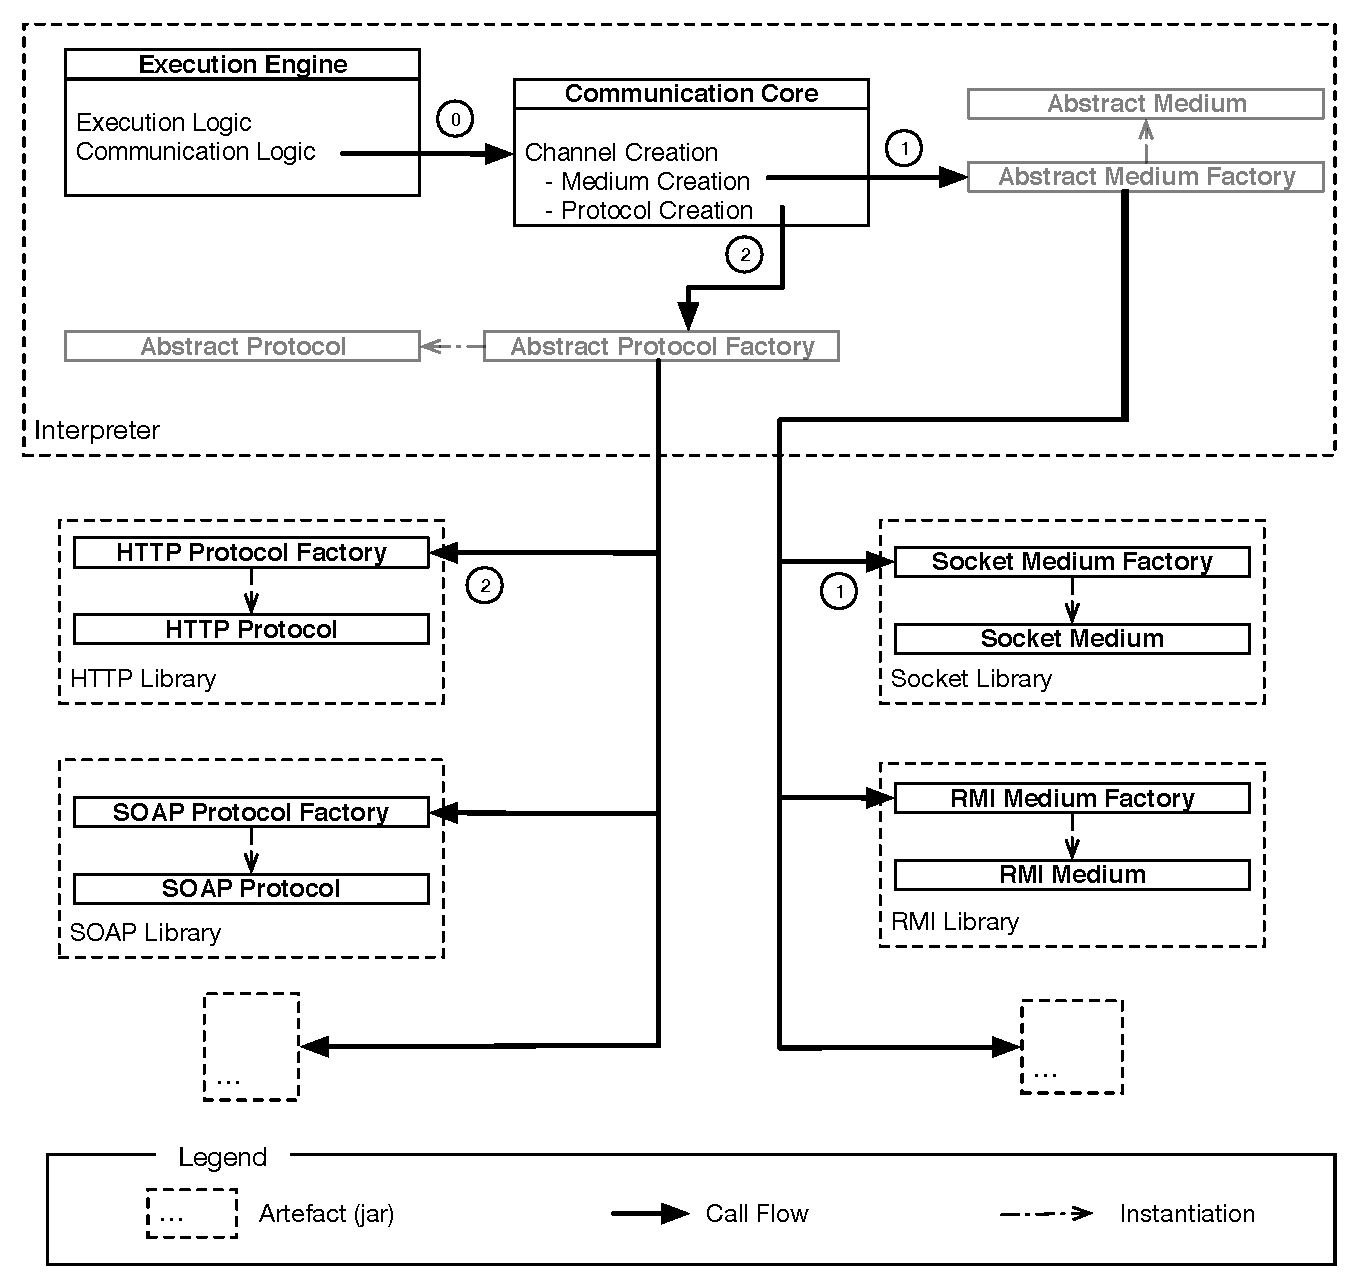
\includegraphics[width=\textwidth]{comm_modules.pdf}
  \caption{Conceptual representation of the call flow among the Jolie
  interpreter and its communication libraries.}
  \label{fig:comm_modules}
\end{figure}

\subsection{Implementation of CoAP/UDP in Jolie} % (fold)
\label{sec:impl_coap_udp}
%
Since by specification the CoAP protocol relies on the UDP medium protocol, in
order to integrate CoAP in Jolie we also had to integrate the UDP medium. As
described in \Cref{sub:jolie_extensions}, this entailed the creation of two
new libraries for the Jolie interpreter: a medium library for UDP and a
protocol library for CoAP.

We remark that, since UDP and CoAP are independent libraries, our 
implementation of UDP can also be used to support other protocols 
relying on UDP, such as MQTT-SN~\cite{hunkeler08}. 
The implementation of UDP consists in a listener and
a sender class, both based on the Netty framework~\cite{maurer16}. Since the
structure expected by Jolie and the one provided by Netty are similar, the
integration of UDP is smooth.
An interesting point is that exceptions raised by Netty are captured and
transformed into JIoT exceptions. These exceptions are notified to the
application protocol, which can either manage them or raise them at the level
of the behavior of the JIoT program.

The implementation of the CoAP library consists in a class taking care of encoding and decoding the message abstraction of Jolie, namely the Communication Message, into a CoAP formatted one. A second class, handling the encoding and decoding of a CoAP message into a buffer of bytes, is based on the work done in nCoAP~\cite{ncoap}, an open source project providing a CoAP implementation for Java, based itself on Netty.

We notice that CoAP supports request-response communications and, in 
particular, CoAP messages include fields \emph{i}) to specify 
at which address the reply is
expected and \emph{ii}) to match a reply with a previous request. Hence, the
implementation of \code{RequestResponse} communications in CoAP is sound also
with a transport protocol which is not connection-oriented, such as UDP.\@ This
would be a problem for protocols that do not provide such a facility, such as
HTTP, which is indeed not commonly used over UDP.

Notably, Jolie comes with a formal semantics (in terms of a process
calculus)~\cite{Guidi2006}, which enables to rigorously reason on the behavior
of Jolie programs. This has been instrumental in the evolution of the language,
e.g., to specify and prove properties on the fault handling mechanisms of the
language~\cite{GuidiLMZ09} or to correctly implement sessions~\cite{MontesiC11}
based on correlation mechanisms~\cite{bpel}. The semantics in~\cite{Guidi2006}
only considers reliable communications and needs to be extended to also cover
the unreliable case. We do not report here on this topic, since it is not
central for the purpose of this paper.

\subsection{Implementation of MQTT in Jolie.} % (fold)
\label{sub:impl_mqtt}

By specification, MQTT relies on the TCP/IP protocol, already implemented in
Jolie. This means that, theoretically, the implementation of MQTT would have
only entailed the creation of a dedicated MQTT protocol library. However, as
detailed in \Cref{sub:jolie_extensions}, Jolie assumes an end-to-end
communication pattern where the caller initiates the creation of a
communication channel with a server, which in turn listens for such inbound
requests. For this reason, given a certain medium, \code{inputPort}s and
\code{outputPort}s use a medium-specific implementation of, respectively, a
listener class and a sender class.
%
This pattern, separating listeners from senders, does not apply to
publish/subscribe protocols, where both the subscriber and the publisher need
to establish a connection with the broker. In our implementation, we mediated
between the two approaches with a Publish-Subscribe medium, which is
essentially a wrapper implementing the logic of Publish-Subscribe message
handling on any other point-to-point medium available (TCP socket in the case
of MQTT) to the interpreter. Although we strove to separate the concerns
between the Jolie interpreter and this new Public-Subscribe channel, we had to
introduce a minimal update into the Jolie Communication Core so that it could
choose between the standard end-to-end media and the new wrapper.

The MQTT protocol class both encodes and decodes messages and implements the QoS
policies of the MQTT standard. Concretely, as for CoAP, we based the
implementation of MQTT on Netty~\cite{maurer16}. The main difficulty in the
implementation of the protocol is the definition of the message patterns needed
to implement \code{OneWay} and \code{RequestResponse} communications, which have
been described in \Cref{sub:mqtt}. Beyond being invoked when operations are executed, the
MQTT class is also invoked when the program is started, to perform port
initialization. In particular, this is when subscriptions to topics identified
in \code{inputPort}s are performed (along with the related connections to the
Brokers).
